\documentclass{bioinfo}
\copyrightyear{2013}
\pubyear{2013}

\begin{document}
\firstpage{1}

\title[iview]{iview: WebGL Visualizer of Protein-Ligand Complex}
\author[Hongjian Li \textit{et~al}]{Hongjian Li\,$^{1,}$\footnote{to whom correspondence should be addressed}, Takanori Nakane\,$^{2}$, Kwong-Sak Leung\,$^{1}$ and Man-Hon Wong\,$^{1}$}
\address{$^{1}$Department of Computer Science and Engineering, Chinese University of Hong Kong, Hong Kong\\
$^{2}$Graduate School of Medicine, Kyoto University, Japan}

\history{Received on XXXXX; revised on XXXXX; accepted on XXXXX}

\editor{Associate Editor: XXXXXXX}

\maketitle

\begin{abstract}

\section{Motivation:}

\section{Results:}

\section{Availability:}
http://istar.cse.cuhk.edu.hk/iview

\section{Contact:} \href{JackyLeeHongJian@Gmail.com}{JackyLeeHongJian@Gmail.com}, \href{nakane.t@gmail.com}{nakane.t@gmail.com}
\end{abstract}

\section{Introduction}

Visualization of protein-ligand complex plays an important role in elaborating protein-ligand interactions and aiding novel drug design. To date, dozens of visualization tools already exist. PyMOL \citep{1221}, Chimera \citep{1219} and VMD \citep{1220} are very well-known and highly cited. They can interpret multiple file formats and generate multiple representations to provide users with precise and powerful control. AutoDockTools4 \citep{596} provides native support for the PDBQT file format, which is widely used in various protein-ligand docking software such as AutoDock \citep{596}, AutoDock Vina \citep{595}, and our idock \citep{1153}. A case study \citep{1321} is presented to process large amounts of geometry data for real-time 3D exploration, superimposition, and interactive navigational tasks in a virtual reality environment. We also developed our own program \citep{1265} to visualize structures in virtual reality settings and employ fragment-based \textit{de novo} ligand design strategy for interactive drug design. LigPlot+ \citep{951} and PoseView \citep{748}, on the other hand, plot 2D diagrams of protein-ligand interactions from 3D coordinates.

In addition, there are web tools based on either Java applet, Flash, or HTML5 canvas. Jmol \citep{1263}, an open source Java viewer for chemical structures in 3D, has been deployed worldwide and recognized as the \textit{de facto} molecular viewer on the web. JSmol \citep{1314}, a JavaScript-only version of Jmol, includes the full implementation of the entire set of Jmol functionalities. GLmol \citep{1319}, a molecular viewer on WebGL/Javascript, supports multiple file formats and representations and features an experimental version of molecular surface based on the EDTSurf algorithm \citep{1297}. Another study \citep{1262} also presents a WebGL technology for rendering molecular surface using the SpiderGL library \citep{1320} ChemDoodle Web Components \citep{1264}, a pure Javascript chemical graphics and cheminformatics library, presents 2D and 3D graphics and animations for chemical structures, reactions and spectra. ePlant \citep{1242}, a suite of open-source Flash-based web tools, visualizes integrative systems biology from the model organism \textit{Arabidopsis thaliana}. PLI \citep{1288} is a web-based tool for the comparison of protein-ligand interactions observed on PDB structures. BioJS \citep{1308} is an open source JavaScript framework for biological data visualization. There is a review that covers a history of web-based structure input \citep{1243}.

However, there is easy-to-use online visualizer. We develop iview, an interactive WebGL visualizer of protein-ligand complex (Figure \ref{istar:iview}). iview is refactored from GLmol 0.47 \citep{1319}.

Modern browsers nowadays, e.g. Chrome, Firefox, Safari and Opera, support WebGL. IE11 will support WebGL too.

4MBS \citep{1348}

\section{Approach}

\begin{methods}
\section{Methods}

Load structure from PDB
Camera: perspective, orthographic
Background: black, grey, white
Color by: spectrum, chain, secondary structure, B factor, residue, polarity, atom
Primary structure: line, stick, ball-and-stick, sphere, nothing
Secondary structure: ribbon, strand, cylinder and plate, C alpha trace, nothing
EDTSurf \citep{1297} is an fast algorithm to generating triangulated macromolecular surfaces by Euclidean distance transform.
Protein surface: Van der Waals surface, solvent excluded surface, solvent accessible surface, molecular surface 
Surface opacity
Wireframe
Rotate, translate, zoom in/out, slab with mouse
Export canvas to png

Tailor-made version specifically for idock jobs
Protein and top hit ligands in PDBQT format
Search space in cubic box
Top 100 ligand switch
Putative hydrogen bonds
10 molecular properties
suppliers

\end{methods}

\begin{figure}%[!tpb]
\centerline{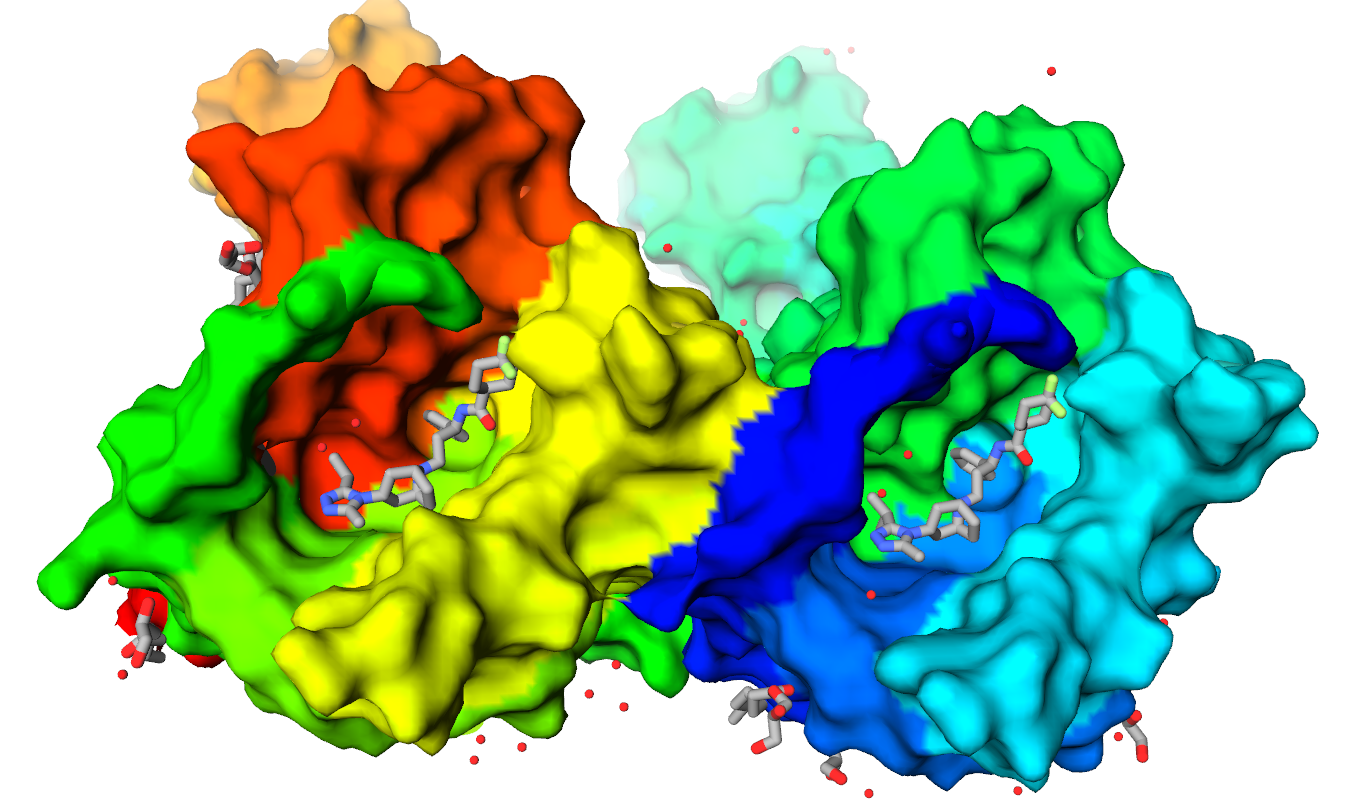
\includegraphics[width=\linewidth]{4MBS.png}}
\caption{iview rendering of the CCR5 chemokine receptor-HIV entry inhibitor maraviroc complex (PDB code: 4MBS). The human CCR5 is rendered as molecular surface colored by spectrum. The marketed HIV drug maraviroc is rendered as stick colored by atom types. It can be clearly seen that the CCR5 forms a deep allosteric cavity where maraviroc is buried.}\label{fig:4MBS}
\end{figure}

\section{Availability}

iview is free and open source under Apache License 2.0. iview is available at http://istar.cse.cuhk.edu.hk/iview. Its source code is available at https://github.com/HongjianLi/istar.

%\section{Conclusion}

%We have developed iview, an interactive WebGL visualizer of protein-ligand complex.

\bibliographystyle{natbib}
%\bibliographystyle{achemnat}
%\bibliographystyle{plainnat}
%\bibliographystyle{abbrv}
%\bibliographystyle{bioinformatics}
%
%\bibliographystyle{plain}

\bibliography{../refworks}

\end{document}
